\documentclass[12pt,a4paper]{article}

% Packages
\usepackage[utf8]{inputenc}
\usepackage[T1]{fontenc}
\usepackage{lmodern}
\usepackage[margin=1in]{geometry}
\usepackage{graphicx}
\usepackage{xcolor}
\usepackage{hyperref}
\usepackage{enumitem}
\usepackage{booktabs}
\usepackage{tabularx}
\usepackage{listings}
\usepackage{float}
\usepackage{amsmath}
\usepackage{tikz}
\usetikzlibrary{shapes.geometric, arrows.meta, positioning}
\usepackage{fancyhdr}
\usepackage{titlesec}

% Colors
\definecolor{ariablue}{HTML}{2563EB}
\definecolor{ariadark}{HTML}{1E293B}
\definecolor{arialight}{HTML}{F1F5F9}
\definecolor{codebg}{HTML}{F8FAFC}
\definecolor{codegreen}{HTML}{16A34A}
\definecolor{codered}{HTML}{DC2626}
\definecolor{codeorange}{HTML}{EA580C}

% Hyperlink setup
\hypersetup{
    colorlinks=true, linkcolor=ariablue, urlcolor=ariablue, citecolor=ariablue
}

% Code listing style
\lstdefinestyle{codestyle}{
    backgroundcolor=\color{codebg}, basicstyle=\ttfamily\small,
    breaklines=true, frame=single, rulecolor=\color{ariablue!30},
    keywordstyle=\color{ariablue}\bfseries, commentstyle=\color{codegreen},
    stringstyle=\color{codered}, tabsize=4
}
\lstset{style=codestyle}

% Header/Footer
\pagestyle{fancy}
\fancyhf{}
\fancyhead[L]{\small\textcolor{ariablue}{ARIA --- Design Document}}
\fancyhead[R]{\small\textcolor{gray}{April 2026}}
\fancyfoot[C]{\thepage}
\renewcommand{\headrulewidth}{0.4pt}

% Title formatting
\titleformat{\section}{\Large\bfseries\color{ariadark}}{}{0em}{}[\titlerule]
\titleformat{\subsection}{\large\bfseries\color{ariablue}}{}{0em}{}
\titleformat{\subsubsection}{\normalsize\bfseries\color{ariadark}}{}{0em}{}

% ============================================================
\begin{document}

% ---------- TITLE PAGE ----------
\begin{titlepage}
    \centering
    \vspace*{2cm}
    {\Huge\bfseries\textcolor{ariadark}{ARIA}}\\[0.5cm]
    {\LARGE\textcolor{ariablue}{Adaptive Review Intelligence Architecture}}\\[1.5cm]
    {\Large\textbf{System Design Document}}\\[0.5cm]
    {\large Version 1.0}\\[2cm]
    \begin{tabular}{ll}
        \textbf{Project:} & Automatic Code Reviewer \\
        \textbf{Theme:} & Multi-LLM Intelligent Code Review \\
        \textbf{Date:} & April 2026 \\
        \textbf{Course:} & Design Lab \\
    \end{tabular}
    \vfill
    {\small\textcolor{gray}{A multi-LLM code review system with cross-model debate verification.}}
\end{titlepage}

\tableofcontents
\newpage

% ============================================================
\section{Executive Summary}
% ============================================================

ARIA (\textbf{A}daptive \textbf{R}eview \textbf{I}ntelligence \textbf{A}rchitecture) accepts a GitHub repository URL and generates a structured code review report using multiple LLM families. Its core innovation is the \textbf{Model Debate Protocol}: specialized agents from different model families (Llama, Gemini, Mistral) independently review code, then cross-verify each other's findings. Only consensus-backed issues surface in the final report, eliminating hallucinations and false positives.

\subsection{Design Goals}
\begin{enumerate}[label=\textbf{G\arabic*.}]
    \item \textbf{Multi-Model Diversity}: Three LLM families to eliminate single-model bias.
    \item \textbf{High Signal-to-Noise}: Cross-verification filters unconfirmed findings.
    \item \textbf{Deep Context}: Repository-level analysis via AST parsing and knowledge graphs.
    \item \textbf{Structured Output}: Severity-ranked findings with line-level annotations and fix suggestions.
    \item \textbf{Zero Cost}: Entirely free-tier APIs.
\end{enumerate}

% ============================================================
\section{Problem Statement}
% ============================================================

AI copilots generate code faster than humans can review it. Single-model reviewers produce 70--80\% noise, and the c-CRAB benchmark shows the best agents solve only $\sim$40\% of complex review tasks. 38.1\% of developers cite AI-generated technical debt (``AI Slop'') as their primary concern. No existing tool cross-verifies findings across independent model families.

\begin{quote}
\textit{Given a GitHub repository URL, design a system that leverages multiple LLM families to produce cross-verified, severity-ranked code review findings with minimal false positives.}
\end{quote}

% ============================================================
\section{Gap Analysis}
% ============================================================

\begin{table}[H]
\centering
\caption{ARIA vs.\ Existing Platforms}
\begin{tabularx}{\textwidth}{lcccc}
\toprule
\textbf{Feature} & \textbf{CodeRabbit} & \textbf{Claude CR} & \textbf{BitsAI} & \textbf{ARIA} \\
\midrule
Multi-model families & \texttimes & \texttimes & \texttimes & \checkmark \\
Cross-model debate & \texttimes & \texttimes & \texttimes & \checkmark \\
Confidence scoring & Partial & Partial & \checkmark & \checkmark \\
Full repo context (AST) & \texttimes & Partial & Partial & \checkmark \\
AI-Slop detection & \texttimes & \texttimes & \texttimes & \checkmark \\
Free / open-source & \texttimes & \texttimes & \texttimes & \checkmark \\
\bottomrule
\end{tabularx}
\end{table}

% ============================================================
\section{System Architecture}
% ============================================================

\subsection{Five-Stage Pipeline}

\begin{figure}[H]
\centering
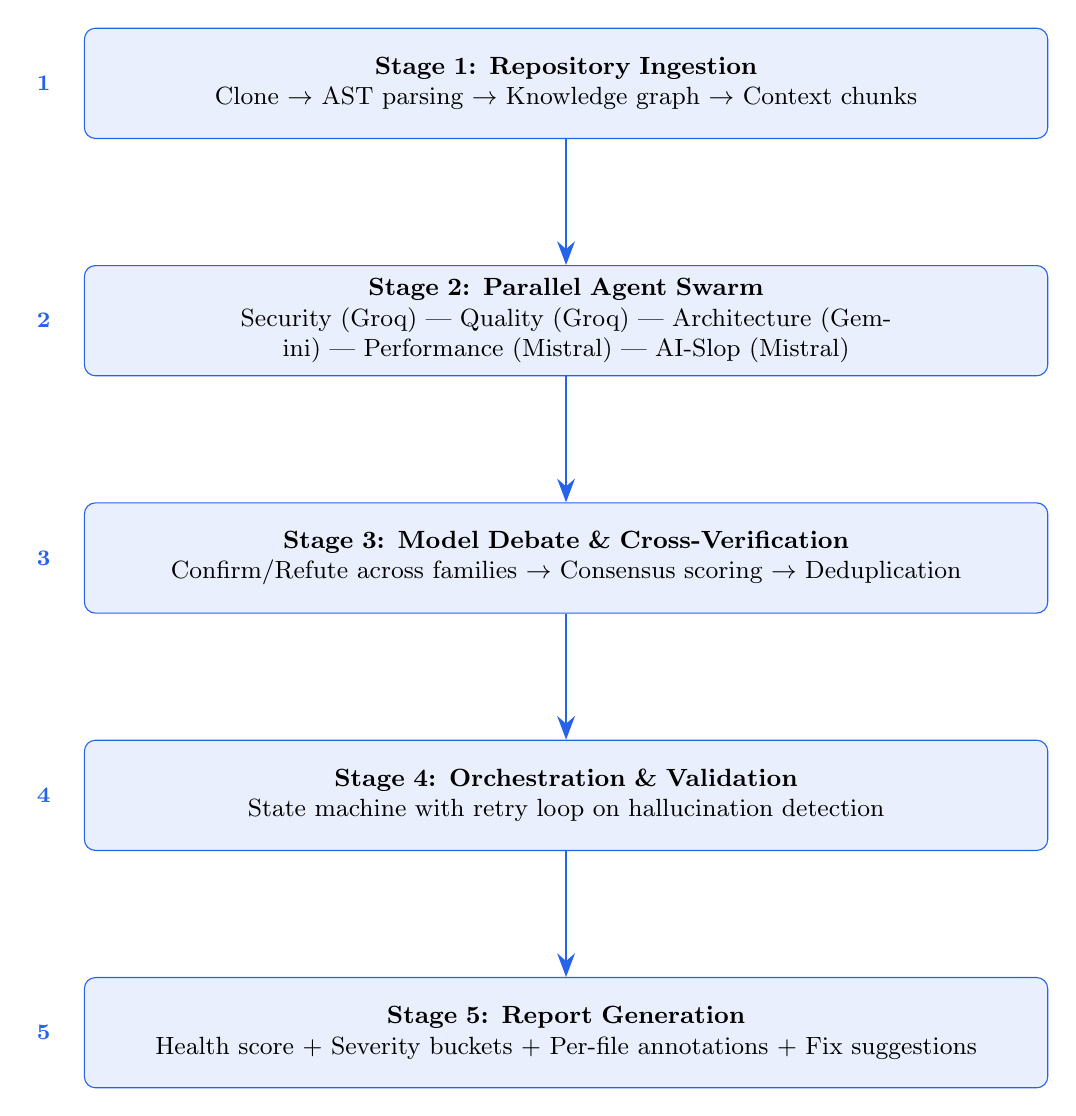
\begin{tikzpicture}[
    node distance=1.6cm,
    stage/.style={rectangle, rounded corners, draw=ariablue, fill=ariablue!10, text width=12cm, minimum height=1.4cm, align=center, font=\small},
    arrow/.style={-{Stealth[length=3mm]}, thick, ariablue},
    label/.style={font=\footnotesize\bfseries, ariablue}
]
\node[stage] (s1) {\textbf{Stage 1: Repository Ingestion}\\Clone $\rightarrow$ AST parsing $\rightarrow$ Knowledge graph $\rightarrow$ Context chunks};
\node[stage, below=of s1] (s2) {\textbf{Stage 2: Parallel Agent Swarm}\\Security (Groq) | Quality (Groq) | Architecture (Gemini) | Performance (Mistral) | AI-Slop (Mistral)};
\node[stage, below=of s2] (s3) {\textbf{Stage 3: Model Debate \& Cross-Verification}\\Confirm/Refute across families $\rightarrow$ Consensus scoring $\rightarrow$ Deduplication};
\node[stage, below=of s3] (s4) {\textbf{Stage 4: Orchestration \& Validation}\\State machine with retry loop on hallucination detection};
\node[stage, below=of s4] (s5) {\textbf{Stage 5: Report Generation}\\Health score + Severity buckets + Per-file annotations + Fix suggestions};
\draw[arrow] (s1)--(s2); \draw[arrow] (s2)--(s3); \draw[arrow] (s3)--(s4); \draw[arrow] (s4)--(s5);
\node[label, left=0.3cm of s1] {1};
\node[label, left=0.3cm of s2] {2};
\node[label, left=0.3cm of s3] {3};
\node[label, left=0.3cm of s4] {4};
\node[label, left=0.3cm of s5] {5};
\end{tikzpicture}
\caption{ARIA Pipeline Architecture}
\end{figure}

\subsection{Agent Specifications}

\begin{table}[H]
\centering
\caption{Specialized Review Agents}
\begin{tabularx}{\textwidth}{llXl}
\toprule
\textbf{Agent} & \textbf{Provider / Model} & \textbf{Focus Area} & \textbf{Dimension} \\
\midrule
Security Auditor & Groq / Llama 3.3 70B & OWASP Top 10, CVEs, hardcoded secrets, injections & Security \\
Code Quality & Groq / Llama 3.3 70B & Complexity, dead code, duplication, error handling & Maintainability \\
Architecture & Gemini 2.0 Flash & SOLID violations, coupling, design patterns & Structure \\
Performance & Mistral Small & O(n\textsuperscript{2}) algorithms, N+1 queries, memory leaks & Performance \\
AI-Slop Detector & Mistral Small & Over-abstraction, brittle AI-generated patterns & Legibility \\
\bottomrule
\end{tabularx}
\end{table}

% ============================================================
\section{Model Debate Protocol}
% ============================================================

The core innovation. After parallel agent review:

\begin{enumerate}
    \item Each finding is serialized as structured JSON (file, line, severity, reasoning).
    \item Each finding is sent to \textbf{2 agents from different model families} for cross-verification.
    \item Verifiers respond with \texttt{CONFIRM} (with evidence) or \texttt{REFUTE} (with counter-reasoning).
    \item Consensus scoring:
    \begin{itemize}
        \item 3/3 confirm $\rightarrow$ confidence 1.0
        \item 2/3 confirm $\rightarrow$ confidence 0.7
        \item 1/3 confirm $\rightarrow$ confidence 0.3 (filtered out)
    \end{itemize}
    \item Cosine similarity deduplication merges overlapping findings (threshold $> 0.85$).
\end{enumerate}

$$C(f) = \frac{\sum_{i=1}^{n} v_i(f)}{n}, \quad v_i \in \{0, 1\}, \quad \text{threshold: } C(f) \geq 0.7$$

\begin{table}[H]
\centering
\caption{Debate Protocol vs.\ Single-Model Review}
\begin{tabularx}{\textwidth}{lXX}
\toprule
\textbf{Failure Mode} & \textbf{Single-Model} & \textbf{ARIA Debate} \\
\midrule
Hallucinated finding & Surfaces to developer & Refuted by other models $\rightarrow$ filtered \\
Missed vulnerability & Never caught & Different family catches it \\
False positive & Wastes developer time & Cross-verification rejects it \\
Model bias & Persists systematically & Uncorrelated biases cancel out \\
\bottomrule
\end{tabularx}
\end{table}

% ============================================================
\section{AI-Slop Detection}
% ============================================================

A dedicated agent addressing the \#1 developer concern in 2026. Detection heuristics:

\begin{enumerate}
    \item \textbf{Over-abstraction}: Unnecessary wrappers, factory patterns for single-use objects
    \item \textbf{Cargo-cult patterns}: Design patterns applied without justification
    \item \textbf{Suspicious uniformity}: Identically structured code across unrelated modules
    \item \textbf{Missing error paths}: Happy-path-only code with no edge case handling
    \item \textbf{Comment-code mismatch}: Generic docstrings that don't match implementation
\end{enumerate}

$$S_{\text{slop}} = \frac{\text{Files flagged}}{\text{Total files}} \times 100$$

$S < 15\%$: \textcolor{codegreen}{\textbf{Low risk}} \quad
$15\% \leq S < 35\%$: \textcolor{codeorange}{\textbf{Moderate}} \quad
$S \geq 35\%$: \textcolor{codered}{\textbf{High risk}}

% ============================================================
\section{Technology Stack}
% ============================================================

\begin{table}[H]
\centering
\caption{Technology Stack}
\begin{tabularx}{\textwidth}{lXl}
\toprule
\textbf{Component} & \textbf{Technology} & \textbf{Purpose} \\
\midrule
Orchestration & LangGraph & State machine with retry loops \\
LLM: Security + Quality & Groq API (Llama 3.3 70B) & Fast, free inference \\
LLM: Architecture & Google Gemini 2.0 Flash & Free tier, strong reasoning \\
LLM: Performance + Slop & Mistral AI (Mistral Small) & Free tier, different family \\
AST Parsing & Regex-based multi-language & Function/class/import extraction \\
Knowledge Graph & NetworkX & Dependency and call graph \\
Deduplication & Jaccard similarity & Finding dedup (threshold 0.85) \\
Backend API & FastAPI & REST endpoints \\
Frontend UI & Streamlit & Web interface \\
Report Rendering & Jinja2 & HTML report generation \\
Language & Python 3.11+ & Primary language \\
\bottomrule
\end{tabularx}
\end{table}

% ============================================================
\section{API Design}
% ============================================================

\begin{table}[H]
\centering
\caption{REST Endpoints}
\begin{tabularx}{\textwidth}{llX}
\toprule
\textbf{Method} & \textbf{Endpoint} & \textbf{Description} \\
\midrule
POST & \texttt{/api/review} & Submit GitHub URL; returns job ID \\
GET & \texttt{/api/review/\{job\_id\}} & Job status and results \\
GET & \texttt{/api/review/\{job\_id\}/report} & Download report (HTML/JSON) \\
GET & \texttt{/api/health} & System health check \\
\bottomrule
\end{tabularx}
\end{table}

\subsection{Health Score Formula}

$$H = \max\!\Big(0,\ 100 - \big(10 \cdot n_{\text{crit}} + 5 \cdot n_{\text{high}} + 2 \cdot n_{\text{med}} + 0.5 \cdot n_{\text{low}}\big)\Big)$$

% ============================================================
\section{Evaluation Strategy}
% ============================================================

\begin{table}[H]
\centering
\caption{Evaluation Metrics}
\begin{tabularx}{\textwidth}{lXl}
\toprule
\textbf{Metric} & \textbf{Methodology} & \textbf{Target} \\
\midrule
Precision & Findings confirmed as true issues by manual audit & $> 70\%$ \\
Consensus Quality & Findings surviving cross-verification & $> 60\%$ \\
False Positive Rate & Findings flagged incorrect by human review & $< 15\%$ \\
Coverage & Known issues (seeded bugs) detected & $> 50\%$ \\
Debate Effectiveness & FP reduction: debate vs.\ no-debate & $> 40\%$ \\
\bottomrule
\end{tabularx}
\end{table}

% ============================================================
\section{Risk Analysis}
% ============================================================

\begin{table}[H]
\centering
\caption{Risk Matrix}
\begin{tabularx}{\textwidth}{lllX}
\toprule
\textbf{Risk} & \textbf{Likelihood} & \textbf{Impact} & \textbf{Mitigation} \\
\midrule
API rate limiting & High & Medium & Exponential backoff; provider rotation \\
Gemini quota exhaust & Medium & Low & Fallback to Groq \\
Large repo overflow & Medium & High & Context windowing; file chunking \\
Hallucinated findings & Medium & High & Model Debate Protocol \\
\bottomrule
\end{tabularx}
\end{table}

% ============================================================
\section{References}
% ============================================================

\begin{enumerate}[label={[\arabic*]}]
    \item ByteDance, ``BitsAI-CR: Industrial-Scale Code Review,'' \textit{arXiv}, 2025.
    \item Anthropic, ``Claude Code Review --- Multi-Agent Architecture,'' 2026.
    \item Qodo, ``The Four Principles of AI Code Governance,'' 2026.
    \item c-CRAB, ``Executable Evaluation for Review Agents,'' 2026.
    \item Alibaba, ``AACR-Bench: Repository-Level Code Review Benchmark,'' 2026.
    \item LangGraph Documentation, ``State Machine Orchestration for LLM Agents,'' 2026.
    \item OWASP, ``Top 10 Web Application Security Risks,'' 2025 Edition.
\end{enumerate}

\end{document}
